\documentclass[main.tex]{subfiles}
\begin{document}

\chapter{The EM Algorithm and Generalised Linear Models}\label{ch:em-glm}\chaptermark{The EM Algorithm and GLMs}

When the maximum likelihood principle (Chapters~\ref{ch:mle}--\ref{ch:mle-asimptotik}) does not give a closed-form solution, the MLE is found numerically. This chapter deals with the two numerical MLE problems met most often in statistics and with the algorithms specific to them. The first is \emph{missing data\index{missing data@missing data}} problems: mixture\index{mixture distribution@mixture distribution} models, censored observations, latent variables. In these, the likelihood is a sum or integral over unobserved variables. The EM algorithm\index{em algorithm@EM algorithm} of Dempster, Laird and Rubin \cite{dempster77} turns the observation ``the problem would be easy if the missing data were known'' into an iterative method that increases the likelihood at every step. The second is \emph{generalised linear\index{generalised linear model glm@generalised linear model (GLM)} models} (GLMs) \cite{nelder-wedderburn72}: the generalisation of the linear model of Chapter~\ref{ch:dogrusal} to binary, count and positive continuous responses. Here Fisher scoring\index{fisher scoring@Fisher scoring} becomes the IRLS\index{irls@IRLS} algorithm, each step of which is a weighted LS problem. Both topics show the computational power of exponential family\index{exponential family@exponential family} structure (Chapter~\ref{ch:yeterlilik}).

\section{Definitions}

\begin{definition}[Missing Data Structure and the $Q$ Function]\label{def:em}
Let $\x$ be the observed data and $\mathbf z$ the unobserved (missing or latent) data; let the density of the \emph{complete data} $(\x,\mathbf z)$ be $f_c(\x,\mathbf z;\theta)$, and that of the observed data $f(\x;\theta)=\int f_c(\x,\mathbf z;\theta)\,d\mathbf z$. The observed-data and complete-data log-likelihoods\index{log likelihood@log-likelihood} are $\ell(\theta)=\ln f(\x;\theta)$ and $\ell_c(\theta)=\ln f_c(\x,\mathbf z;\theta)$. The conditional density of the missing data\index{missing data@missing data} is $k(\mathbf z\mid\x;\theta)=f_c(\x,\mathbf z;\theta)/f(\x;\theta)$.
\[
Q(\theta\mid\theta')=\E_{\theta'}\big[\ell_c(\theta;\x,\mathbf Z)\,\big|\,\x\big],\qquad H(\theta\mid\theta')=\E_{\theta'}\big[\ln k(\mathbf Z\mid\x;\theta)\,\big|\,\x\big].
\]
\end{definition}

\begin{definition}[The EM Algorithm]\label{def:em-algoritma}\index{em algorithm@EM algorithm|textbf}
Starting from an initial $\theta^{(0)}$, for $t=0,1,2,\dots$:
\begin{itemize}
  \item \emph{E-step:} compute $Q(\theta\mid\theta^{(t)})$ (find the conditional expectations\index{conditional expectation@conditional expectation} of the sufficient statistics\index{sufficient statistic@sufficient statistic} of the missing data).
  \item \emph{M-step:} $\theta^{(t+1)}=\argmax_\theta Q(\theta\mid\theta^{(t)})$.
\end{itemize}
If instead of full maximisation the M-step only ensures $Q(\theta^{(t+1)}\mid\theta^{(t)})\ge Q(\theta^{(t)}\mid\theta^{(t)})$, the algorithm is called \emph{generalised EM} (GEM).
\end{definition}

\begin{definition}[Exponential Dispersion Family]\label{def:ustel-dagilim}
Densities (or probability mass functions) of the form
\[
f(y;\theta,\phi)=\exp\Big\{\frac{y\theta-b(\theta)}{a(\phi)}+c(y,\phi)\Big\}
\]
are called an \emph{exponential dispersion family\index{exponential dispersion family@exponential dispersion family}}; $\theta$ is the natural (canonical) parameter and $\phi$ the dispersion parameter. If $\phi$ is known, this is a one-parameter exponential family\index{exponential family@exponential family} with sufficient statistic $T(y)=y$.
\end{definition}

\begin{definition}[Generalised Linear Model]\label{def:glm}
Let $Y_1,\dots,Y_n$ be independent, each from an exponential dispersion family; $\mu_i=\E Y_i$. A GLM\index{generalised linear model glm@generalised linear model (GLM)} has three components:
\begin{enumerate}
  \item \emph{Random component:} the distribution of $Y_i$ in the exponential dispersion family;
  \item \emph{Linear predictor:} $\eta_i=\mathbf x_i^\top\bm\beta$;
  \item \emph{Link function\index{link function@link function}:} $g(\mu_i)=\eta_i$ with $g$ monotone and differentiable.
\end{enumerate}
If $g=(b')^{-1}$, i.e.\ $\theta_i=\eta_i$, then $g$ is called the \emph{canonical link}. $V(\mu)=b''(\theta(\mu))$ is called the \emph{variance function}.
\begin{center}
\begin{tabular}{lcccc}
\toprule
Distribution & $b(\theta)$ & $V(\mu)$ & $a(\phi)$ & Canonical link\\
\midrule
$\Normal(\mu,\sigma^2)$ & $\theta^2/2$ & $1$ & $\sigma^2$ & identity\\
$\text{Bernoulli}(\mu)$ & $\ln(1+e^\theta)$ & $\mu(1-\mu)$ & $1$ & logit $\ln\frac{\mu}{1-\mu}$\\
$\text{Poisson}(\mu)$ & $e^\theta$ & $\mu$ & $1$ & $\ln\mu$\\
$\text{Gamma}$ (shape $\nu$, mean $\mu$) & $-\ln(-\theta)$ & $\mu^2$ & $1/\nu$ & $-1/\mu$\\
\bottomrule
\end{tabular}
\end{center}
\end{definition}

\begin{definition}[Deviance]\label{def:sapma}\index{deviance@deviance|textbf}
Let $\ell_{\text{sat}}$ be the log-likelihood of the (\emph{saturated}) model that gives each observation its own mean. $D=2a(\phi)\big[\ell_{\text{sat}}-\ell(\hat{\bm\beta})\big]$ is called the \emph{deviance}, and $D/a(\phi)$ the \emph{scaled deviance}. In the normal model $D=\mathrm{SSE}$; the deviance is the GLM counterpart of the residual sum of squares. In the Bernoulli model $D=2\sum_i\big[y_i\ln\frac{y_i}{\hat\mu_i}+(1-y_i)\ln\frac{1-y_i}{1-\hat\mu_i}\big]$ ($0\ln0=0$).
\end{definition}

\section{Main Theorems and Proofs}

\begin{theorem}[Monotonicity of EM \cite{dempster77}]\label{thm:em-monoton}\index{em algorithm@EM algorithm}
For the EM (and GEM) sequence, $\ell(\theta^{(t+1)})\ge\ell(\theta^{(t)})$. Equality holds only if $Q(\theta^{(t+1)}\mid\theta^{(t)})=Q(\theta^{(t)}\mid\theta^{(t)})$ and $k(\cdot\mid\x;\theta^{(t+1)})=k(\cdot\mid\x;\theta^{(t)})$ a.e.
\end{theorem}
\begin{proof}
For every $\mathbf z$, $\ell(\theta)=\ell_c(\theta;\x,\mathbf z)-\ln k(\mathbf z\mid\x;\theta)$. The left-hand side does not depend on $\mathbf z$; taking the expectation of both sides under $k(\cdot\mid\x;\theta')$,
\[
\ell(\theta)=Q(\theta\mid\theta')-H(\theta\mid\theta')\qquad\text{for all }\theta,\theta'.
\]
Applying the information inequality\index{information inequality@information inequality} (Lemma~\ref{lem:bilgi-esitsizligi}) to two conditional densities for the same $\x$,
\[
H(\theta\mid\theta')-H(\theta'\mid\theta')=\E_{\theta'}\Big[\ln\frac{k(\mathbf Z\mid\x;\theta)}{k(\mathbf Z\mid\x;\theta')}\,\Big|\,\x\Big]\le\ln\E_{\theta'}\Big[\frac{k(\mathbf Z\mid\x;\theta)}{k(\mathbf Z\mid\x;\theta')}\,\Big|\,\x\Big]\le0,
\]
i.e.\ $H(\cdot\mid\theta')$ attains its maximum at $\theta'$ (Jensen\index{jensen s inequality@Jensen's inequality}; with equality only if the two conditional densities are equal a.e.). With $\theta'=\theta^{(t)}$ and $\theta=\theta^{(t+1)}$,
\[
\ell(\theta^{(t+1)})-\ell(\theta^{(t)})=\underbrace{\big[Q(\theta^{(t+1)}\mid\theta^{(t)})-Q(\theta^{(t)}\mid\theta^{(t)})\big]}_{\ge0\ \text{(M-step)}}-\underbrace{\big[H(\theta^{(t+1)}\mid\theta^{(t)})-H(\theta^{(t)}\mid\theta^{(t)})\big]}_{\le0}\ \ge0 .
\qedhere
\]
\end{proof}

% <<fig:em-alt-sinir>>
The geometric content of the proof can be seen in Figure~\ref{fig:em-alt-sinir}.

\begin{figure}[ht]
\centering
\begin{tikzpicture}[x=1.6cm,y=1.1cm,font=\small]
\draw[->] (0,0) -- (5.6,0) node[below] {$\theta$}; \draw[->] (0,0) -- (0,3.6);
\draw[very thick,blue!60!black] (0.200,-0.150) -- (0.288,0.032) -- (0.376,0.209) -- (0.464,0.381) -- (0.553,0.547) -- (0.641,0.707) -- (0.729,0.863) -- (0.817,1.012) -- (0.905,1.157) -- (0.993,1.296) -- (1.081,1.429) -- (1.169,1.557) -- (1.258,1.680) -- (1.346,1.797) -- (1.434,1.908) -- (1.522,2.015) -- (1.610,2.115) -- (1.698,2.211) -- (1.786,2.301) -- (1.875,2.385) -- (1.963,2.464) -- (2.051,2.538) -- (2.139,2.606) -- (2.227,2.669) -- (2.315,2.726) -- (2.403,2.778) -- (2.492,2.824) -- (2.580,2.865) -- (2.668,2.901) -- (2.756,2.931) -- (2.844,2.956) -- (2.932,2.975) -- (3.020,2.989) -- (3.108,2.997) -- (3.197,3.000) -- (3.285,2.997) -- (3.373,2.990) -- (3.461,2.976) -- (3.549,2.957) -- (3.637,2.933) -- (3.725,2.903) -- (3.814,2.868) -- (3.902,2.828) -- (3.990,2.782) -- (4.078,2.730) -- (4.166,2.673) -- (4.254,2.611) -- (4.342,2.543) -- (4.431,2.470) -- (4.519,2.391) -- (4.607,2.307) -- (4.695,2.218) -- (4.783,2.123) -- (4.871,2.022) -- (4.959,1.917) -- (5.047,1.805) -- (5.136,1.689) -- (5.224,1.567) -- (5.312,1.439) -- (5.400,1.306) node[right] {$\ell(\theta)$};
\draw[thick,orange!80!black] (0.250,-0.167) -- (0.303,-0.035) -- (0.357,0.092) -- (0.410,0.215) -- (0.464,0.334) -- (0.517,0.448) -- (0.570,0.559) -- (0.624,0.665) -- (0.677,0.766) -- (0.731,0.864) -- (0.784,0.957) -- (0.837,1.046) -- (0.891,1.130) -- (0.944,1.210) -- (0.997,1.286) -- (1.051,1.358) -- (1.104,1.426) -- (1.158,1.489) -- (1.211,1.548) -- (1.264,1.602) -- (1.318,1.653) -- (1.371,1.699) -- (1.425,1.741) -- (1.478,1.778) -- (1.531,1.812) -- (1.585,1.841) -- (1.638,1.865) -- (1.692,1.886) -- (1.745,1.902) -- (1.798,1.914) -- (1.852,1.921) -- (1.905,1.925) -- (1.958,1.924) -- (2.012,1.918) -- (2.065,1.909) -- (2.119,1.895) -- (2.172,1.877) -- (2.225,1.855) -- (2.279,1.828) -- (2.332,1.797) -- (2.386,1.762) -- (2.439,1.723) -- (2.492,1.679) -- (2.546,1.631) -- (2.599,1.579) -- (2.653,1.522) -- (2.706,1.462) -- (2.759,1.396) -- (2.813,1.327) -- (2.866,1.253) -- (2.919,1.176) -- (2.973,1.093) -- (3.026,1.007) -- (3.080,0.916) -- (3.133,0.821) -- (3.186,0.722) -- (3.240,0.618) -- (3.293,0.510) -- (3.347,0.398) -- (3.400,0.282) node[right] {$m(\theta)$};
\draw[dashed,gray] (0.8,0) node[below,black] {$\theta^{(t)}$} -- (0.8,0.984);
\draw[dashed,gray] (1.920,0) node[below,black] {$\theta^{(t+1)}$} -- (1.920,2.427);
\fill (0.8,0.984) circle (1.6pt) (1.920,1.925) circle (1.6pt) (1.920,2.427) circle (1.6pt);
\draw[{Latex}-{Latex},red!60!black] (2.040,1.925) -- (2.040,2.427);
\end{tikzpicture}
\caption{One step of EM. The decomposition in the proof shows that $m(\theta)=Q(\theta\mid\theta^{(t)})-H(\theta^{(t)}\mid\theta^{(t)})$ lies below $\ell(\theta)$ everywhere and touches it at $\theta^{(t)}$. The M-step maximises $m$; hence $\ell(\theta^{(t+1)})\ge m(\theta^{(t+1)})\ge m(\theta^{(t)})=\ell(\theta^{(t)})$. In the next step a new lower bound is built at $\theta^{(t+1)}$, and the likelihood climbs step by step.}\label{fig:em-alt-sinir}
\end{figure}
% <</fig:em-alt-sinir>>

\begin{proposition}[Stationary Points]\label{prop:em-duragan}
Let $\Theta$ be open, let $\ell$ and $Q(\cdot\mid\theta')$ be differentiable, and let differentiation under the integral sign be permitted. For every $\theta'$,
\[
\nabla\ell(\theta')=\nabla_\theta Q(\theta\mid\theta')\big|_{\theta=\theta'} .
\]
Hence a fixed point $\theta^*$ of EM ($\theta^*$ an interior maximum of $Q(\cdot\mid\theta^*)$) is a stationary point of $\ell$.
\end{proposition}
\begin{proof}
$\ell(\theta)=Q(\theta\mid\theta')-H(\theta\mid\theta')$, and since $H(\cdot\mid\theta')$ attains its maximum at the interior point $\theta'$, $\nabla_\theta H(\theta\mid\theta')|_{\theta=\theta'}=0$. Differentiate. At a fixed point $\nabla_\theta Q(\theta^*\mid\theta^*)=0$, hence $\nabla\ell(\theta^*)=0$.
\end{proof}

\begin{remark}[Convergence and Rate]
Monotonicity guarantees convergence of the sequence $\ell(\theta^{(t)})$ if $\ell$ is bounded above. It does not, however, guarantee that $\theta^{(t)}$ converges to the global maximum: under additional continuity conditions the limit points are stationary points \cite{wu83}, which may be local maxima or saddle points. Near a stationary $\theta^*$, EM converges linearly: $\theta^{(t+1)}-\theta^*\approx J(\theta^{(t)}-\theta^*)$, where (in one dimension)
\[
J=\frac{I_{\text{miss}}}{I_{\text{com}}}=1-\frac{I_{\text{obs}}}{I_{\text{com}}},\qquad I_{\text{com}}=-\partial^2_\theta Q(\theta\mid\theta^*)\big|_{\theta^*},\quad I_{\text{obs}}=-\ell''(\theta^*).
\]
$J$ is the \emph{fraction of missing information} \cite{dempster77}: if the missing data\index{missing data@missing data} carry most of the information, EM is slow.
\end{remark}

\begin{proposition}[Moments of the Exponential Dispersion Family]\label{prop:edf-moment}
For the family of Definition~\ref{def:ustel-dagilim}, $\E Y=b'(\theta)$ and $\Var Y=a(\phi)\,b''(\theta)$.
\end{proposition}
\begin{proof}
For $\ell(\theta)=\frac{y\theta-b(\theta)}{a(\phi)}+c(y,\phi)$ the score is $\ell'=\frac{y-b'(\theta)}{a(\phi)}$ and $\ell''=-\frac{b''(\theta)}{a(\phi)}$. By Lemma~\ref{lem:skor}, $\E\ell'=0$, i.e.\ $\E Y=b'(\theta)$. The information identity\index{information identity@information identity} $\E[\ell'^2]=-\E\ell''$ gives $\frac{\Var Y}{a(\phi)^2}=\frac{b''(\theta)}{a(\phi)}$.
\end{proof}

\begin{theorem}[Score and Fisher Information in a GLM]\label{thm:glm-skor}\index{generalised linear model glm@generalised linear model (GLM)}
In a GLM with $\phi$ known,
\begin{gather*}
\mathbf U(\bm\beta)=\nabla_{\bm\beta}\ell=\frac1{a(\phi)}\sum_{i=1}^n\frac{y_i-\mu_i}{V(\mu_i)\,g'(\mu_i)}\,\mathbf x_i,\\
I(\bm\beta)=\frac1{a(\phi)}X^\top WX,\qquad W=\mathrm{diag}\Big(\frac1{V(\mu_i)g'(\mu_i)^2}\Big).
\end{gather*}
For the canonical link\index{link function@link function}, $\mathbf U=\frac1{a(\phi)}X^\top(\mathbf y-\bm\mu)$, the observed information\index{observed information@observed information} equals the expected information ($-\nabla^2\ell=I(\bm\beta)$, independent of the data), and $\ell$ is a concave function of $\bm\beta$; if $X$ has full column rank it is strictly concave.
\end{theorem}
\begin{proof}
Chain rule: $\frac{\partial\ell_i}{\partial\bm\beta}=\frac{\partial\ell_i}{\partial\theta_i}\frac{d\theta_i}{d\mu_i}\frac{d\mu_i}{d\eta_i}\frac{\partial\eta_i}{\partial\bm\beta}$. Here $\frac{\partial\ell_i}{\partial\theta_i}=\frac{y_i-\mu_i}{a(\phi)}$, $\frac{d\mu_i}{d\theta_i}=b''(\theta_i)=V(\mu_i)$, $\frac{d\mu_i}{d\eta_i}=\frac1{g'(\mu_i)}$ and $\frac{\partial\eta_i}{\partial\bm\beta}=\mathbf x_i$. The product gives the score formula. For independent terms the Fisher information\index{fisher information@Fisher information} is $I=\sum_i\Cov(\nabla\ell_i)$, and using $\Var Y_i=a(\phi)V(\mu_i)$ from Proposition~\ref{prop:edf-moment},
\[
I(\bm\beta)=\sum_i\frac{a(\phi)V(\mu_i)}{a(\phi)^2V(\mu_i)^2g'(\mu_i)^2}\mathbf x_i\mathbf x_i^\top=\frac1{a(\phi)}X^\top WX .
\]
For the canonical link $\theta_i=\eta_i$, so $g'(\mu)=d\theta/d\mu=1/V(\mu)$ and the score becomes $\frac1{a(\phi)}\sum(y_i-\mu_i)\mathbf x_i$. Differentiating once more, $-\nabla^2\ell=\frac1{a(\phi)}\sum_ib''(\eta_i)\mathbf x_i\mathbf x_i^\top$; this expression does not involve $y$, equals $I(\bm\beta)$, and is positive semidefinite because $b''=V>0$. If $X$ has full rank, then for every $\mathbf v\ne\mathbf 0$, $\mathbf v^\top X^\top WX\mathbf v=\sum_iW_{ii}(\mathbf x_i^\top\mathbf v)^2>0$.
\end{proof}

\begin{theorem}[Fisher Scoring = Iteratively Reweighted Least Squares]\label{thm:irls}
The Fisher scoring\index{fisher scoring@Fisher scoring} step $\bm\beta^{\text{new}}=\bm\beta+I(\bm\beta)^{-1}\mathbf U(\bm\beta)$ is the same as
\[
\bm\beta^{\text{new}}=(X^\top WX)^{-1}X^\top W\mathbf z,\qquad z_i=\eta_i+(y_i-\mu_i)\,g'(\mu_i),
\]
where $W$, $\eta$, $\mu$ are computed at the current $\bm\beta$. That is, each step is a weighted LS regression of the \emph{working response} $\mathbf z$ on $X$ with weights $W$ (IRLS\index{irls@IRLS}). For the canonical link, Fisher scoring coincides with the Newton--Raphson\index{newton raphson method@Newton--Raphson method} method.
\end{theorem}
\begin{proof}
Since $\frac{y_i-\mu_i}{V(\mu_i)g'(\mu_i)}=W_{ii}\,(y_i-\mu_i)g'(\mu_i)$, $a(\phi)\mathbf U=X^\top W\mathbf r$ with $r_i=(y_i-\mu_i)g'(\mu_i)$. Hence
\[
X^\top WX\,\bm\beta^{\text{new}}=X^\top WX\bm\beta+X^\top W\mathbf r=X^\top W(X\bm\beta+\mathbf r)=X^\top W\mathbf z
\]
($a(\phi)$ cancels). For the canonical link, the observed and expected information are equal (Theorem~\ref{thm:glm-skor}), so the Newton step $\bm\beta-[\nabla^2\ell]^{-1}\mathbf U$ and the Fisher step are the same.
\end{proof}

\begin{corollary}[Asymptotic Inference in GLMs]\label{cor:glm-asimptotik}\index{generalised linear model glm@generalised linear model (GLM)}
Under regularity conditions\index{regularity conditions@regularity conditions} (Chapter~\ref{ch:mle-asimptotik}), $\hat{\bm\beta}\approx\Normal_p\big(\bm\beta,\ a(\phi)(X^\top\hat WX)^{-1}\big)$; Wald intervals\index{wald confidence interval@Wald confidence interval} are constructed as $\hat\beta_j\pm z_{\alpha/2}\,\mathrm{se}(\hat\beta_j)$. For two nested models, the difference of scaled deviances\index{deviance@deviance} $\big(D_0-D_1\big)/a(\phi)$ is $2\ln$ of the likelihood ratio and, by Wilks\index{wilks theorem@Wilks' theorem}' theorem (Theorem~\ref{thm:wilks}), is approximately $\chi^2_{p_1-p_0}$.
\end{corollary}
\begin{proof}
$\hat{\bm\beta}$ is an MLE and $I(\bm\beta)$ is given in Theorem~\ref{thm:glm-skor}. For independent but not identically distributed observations, asymptotic normality\index{asymptotic normality@asymptotic normality} is obtained by checking the Lindeberg condition\index{lindeberg condition@Lindeberg condition}, as in the LS proof of Chapter~\ref{ch:dogrusal}. By definition the deviance difference is $2[\ell(\hat{\bm\beta}_1)-\ell(\hat{\bm\beta}_0)]a(\phi)$, because the $\ell_{\text{sat}}$ terms cancel.
\end{proof}

\section{Worked Examples}

\begin{example}[EM for a Two-Component Normal Mixture]\label{ex:em-karisim}
$X_i\iid(1-w)\Normal(\mu_1,\sigma_1^2)+w\Normal(\mu_2,\sigma_2^2)$. The latent variable $Z_i\in\{0,1\}$ indicates which component $X_i$ comes from. The complete-data log-likelihood\index{log likelihood@log-likelihood}
\[
\ell_c=\sum_i\Big[Z_i\big(\ln w+\ln\phi(x_i;\mu_2,\sigma_2)\big)+(1-Z_i)\big(\ln(1-w)+\ln\phi(x_i;\mu_1,\sigma_1)\big)\Big]
\]
is linear in the $Z_i$. The E-step only computes the \emph{responsibilities} $\gamma_i=\P(Z_i=1\mid x_i;\theta^{(t)})$:
\[
\gamma_i=\frac{w\,\phi(x_i;\mu_2,\sigma_2)}{w\,\phi(x_i;\mu_2,\sigma_2)+(1-w)\,\phi(x_i;\mu_1,\sigma_1)} .
\]
In the M-step, $Q$ is the complete-data log-likelihood with $\gamma_i$ in place of $Z_i$; it gives weighted normal MLEs: $w=\bar\gamma$, $\mu_2=\sum\gamma_ix_i/\sum\gamma_i$, $\sigma_2^2=\sum\gamma_i(x_i-\mu_2)^2/\sum\gamma_i$, and analogues with weights $1-\gamma_i$ for the first component. The mixture\index{mixture distribution@mixture distribution} likelihood is unbounded: with $\mu_1=x_1$ and $\sigma_1\to0$, $\ell\to\infty$. Hence the ``MLE'' must be understood as a sensible local maximum; in practice a lower bound is imposed on the variances or several starting points are tried.
\end{example}

\begin{example}[Genetic Linkage Data \cite{dempster77}]\label{ex:baglanti}
The counts of $197$ animals in four categories are $\mathbf y=(125,18,20,34)$, with probabilities $\big(\frac12+\frac\theta4,\frac{1-\theta}4,\frac{1-\theta}4,\frac\theta4\big)$. The observed log-likelihood is $y_1\ln(2+\theta)+(y_2+y_3)\ln(1-\theta)+y_4\ln\theta$ (up to a constant), and the likelihood equation is a quadratic equation. From the EM\index{em algorithm@EM algorithm} point of view, the first cell is the sum of two latent cells with probabilities $\frac12$ and $\frac\theta4$: $y_1=x_1+x_2$. The complete data have a binomial structure with $(x_2+y_4)$ successes and $(y_2+y_3)$ failures.
\begin{itemize}
  \item E-step: $x_2^{(t)}=y_1\frac{\theta^{(t)}/4}{1/2+\theta^{(t)}/4}$.
  \item M-step: $\theta^{(t+1)}=\frac{x_2^{(t)}+y_4}{x_2^{(t)}+y_2+y_3+y_4}$.
\end{itemize}
\end{example}

\begin{example}[Poisson Regression]\label{ex:poisson-reg}
$Y_i\sim\text{Poisson}(\mu_i)$, $\ln\mu_i=\mathbf x_i^\top\bm\beta$ (canonical link\index{link function@link function}). By Theorem~\ref{thm:glm-skor}, the score equations are $X^\top(\mathbf y-\hat{\bm\mu})=\mathbf 0$. If the model contains an intercept, the first equation is $\sum_iy_i=\sum_i\hat\mu_i$: the total of the fitted counts reproduces the observed total exactly. In IRLS\index{irls@IRLS} $g'(\mu)=1/\mu$, so $W=\mathrm{diag}(\mu_i)$ and $z_i=\eta_i+(y_i-\mu_i)/\mu_i$. $e^{\beta_j}$ is the factor by which a one-unit increase in $x_j$ multiplies the expected count.
\end{example}

\section{Computational Applications}

\subsection{EM: Linkage Data and a Normal Mixture}

\pycode{code/ch23/c23_1_em_mixture_and_linkage.py}
\begin{lstlisting}[style=output]
Linkage data: EM iterations = [0.608247 0.624321 0.626489 0.626777 0.626816 0.626821]
Direct MLE = 0.626821 | successive error ratios = [0.1346 0.133  0.1328 0.1328 0.1328]
Mixture: 121 iterations | log-likelihood -1324.52 -> -859.4867
Smallest increase = 9.89e-11 (non-negative: monotonicity)
Estimates: w = 0.318 (0.35), mu = (0.083, 3.984) (0, 4), sigma = (1.473, 0.903) (1.5, 1)
\end{lstlisting}

\begin{figure}[h]
\centering
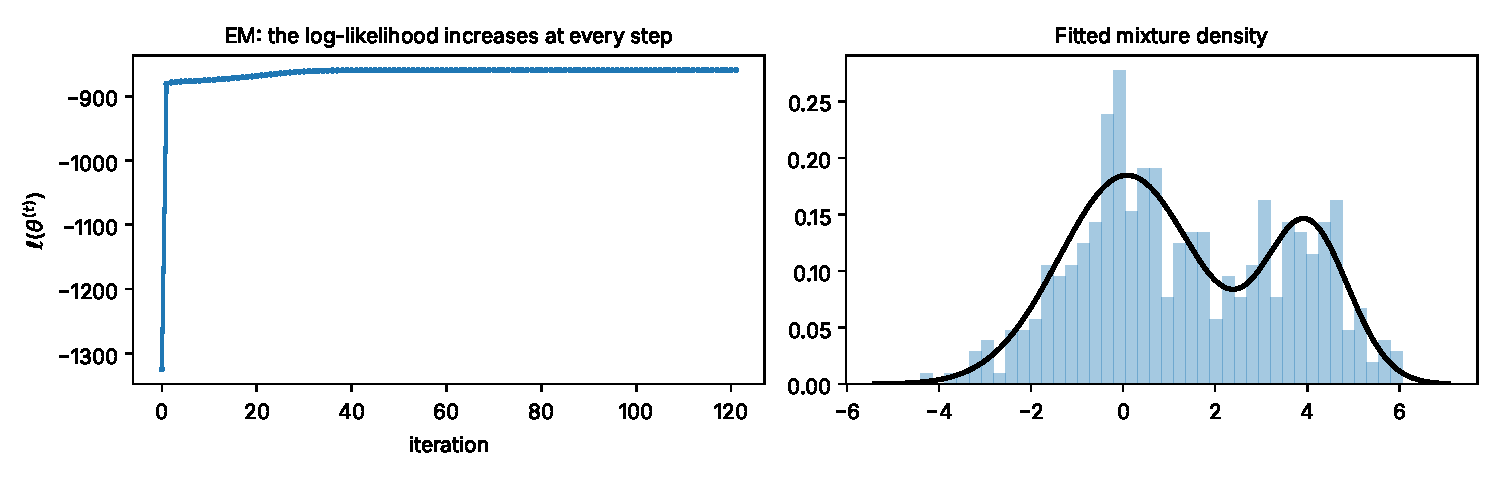
\includegraphics[width=0.95\textwidth]{figures/em_karisim.pdf}
\caption{Left: EM increases the log-likelihood at every step (Theorem~\ref{thm:em-monoton}); a rapid increase after a poor start, followed by slow progress. Right: the fitted two-component mixture density.}
\end{figure}

For the linkage data, EM\index{em algorithm@EM algorithm} reaches the root of the likelihood equation, $\hat\theta=0.626821$, within a few steps. The ratio of successive errors settles at the constant $0.1328$: linear convergence. This ratio equals the fraction of missing information $1-I_{\text{obs}}/I_{\text{com}}$ (Exercise~\ref{exr:23-4}). In the mixture\index{mixture distribution@mixture distribution} example the log-likelihood\index{log likelihood@log-likelihood} decreases at no step; the smallest increase is positive. However, $121$ steps are needed, because the two components partly overlap and the fraction of missing information is high. The estimates are close to the true values. The difference in $w$ ($0.318$ vs $0.35$) is of the usual size of sampling variability at $n=400$.

\subsection{Logistic Regression: IRLS, Wald Intervals and Complete Separation}

\pycode{code/ch23/c23_2_logistic_irls.py}
\begin{lstlisting}[style=output]
IRLS converged in 6 iterations: beta_hat = [-0.4896  1.045  -1.7819]
General-purpose optimiser (BFGS):  beta_hat = [-0.4896  1.045  -1.7819]
Standard errors sqrt(diag((X'WX)^-1)) = [0.1736 0.2156 0.3283]
Deviance = 208.660 | degrees of freedom n - p = 197
Coverage of 95% Wald intervals (M = 2000, n = 200): [0.952 0.958 0.964]
Complete separation,  2 IRLS steps: slope =      2.74 | log-likelihood = -4.69e+00
Complete separation,  4 IRLS steps: slope =      5.79 | log-likelihood = -1.82e+00
Complete separation,  6 IRLS steps: slope =     12.80 | log-likelihood = -5.80e-01
Complete separation,  8 IRLS steps: slope =     26.20 | log-likelihood = -9.13e-02
\end{lstlisting}

IRLS\index{irls@IRLS} reaches the same estimates as a general-purpose optimiser in six steps. Since for the canonical link\index{link function@link function} it is Newton's method (Theorem~\ref{thm:irls}), convergence is quadratic. The coverage of the Wald intervals\index{wald confidence interval@Wald confidence interval} obtained from $(X^\top\hat WX)^{-1}$ is close to the nominal $95\%$ at $n=200$. Although the deviance\index{deviance@deviance} ($208.7$) seems close to the degrees of freedom ($197$), for Bernoulli data this comparison \emph{cannot} be used as a goodness-of-fit\index{goodness of fit@goodness of fit} test. With one trial per observation, the saturated model spends one parameter per observation, and the deviance does not converge to a $\chi^2$ distribution. Deviance differences (Corollary~\ref{cor:glm-asimptotik}), on the other hand, are valid.

The last lines show a situation in which the MLE does not exist. If all observations with $x>0$ are $1$ and those with $x<0$ are $0$ (\emph{complete separation\index{complete separation@complete separation}}), the slope goes to infinity and drives the log-likelihood towards zero; the supremum is not attained at any finite $\bm\beta$. In IRLS the slope roughly doubles at each step, and the algorithm eventually breaks down numerically. Albert and Anderson \cite{albert-anderson84} showed that in logistic regression\index{logistic regression@logistic regression} a finite MLE exists if and only if the data are not completely or quasi-completely separated. In practice penalised likelihood or Bayesian priors are used.

\subsection{Real Data: O-Ring Damage Before Challenger}\label{sec:challenger}
On 28 January 1986 the space shuttle Challenger broke apart 73 seconds after launch. The cause was that the O-rings in the joints of the solid rocket boosters lost their elasticity in the cold. On the night before the launch, engineers discussed the effect of temperature. It is reported that the discussion mostly looked only at the flights on which O-ring damage had been seen. Once the undamaged flights are taken into account, however, the picture changes: all 16 undamaged flights were launched at $66^\circ$F or above, while four of the 7 damaged flights were launched at $63^\circ$F or below. Dalal and colleagues \cite{dalal89} analysed all 23 previous flights with logistic regression. The code fits the model $\operatorname{logit}\P(\text{damage})=\beta_0+\beta_1T$ by the IRLS of Chapter~\ref{ch:em-glm}; it gives the Wald and LRT\index{likelihood ratio test lrt@likelihood ratio test (LRT)} tests of $\beta_1=0$, the odds multiplier for a $10^\circ$F drop, and the damage probability at several temperatures. The temperature forecast for the morning of the launch, and used in the analysis of Dalal and colleagues, is $31^\circ$F (about $-0.6^\circ$C). The probability intervals are built on the logit scale by the delta method\index{delta method@delta method} and transformed back.

\pycode{code/ch23/c23_3_challenger_real_data.py}
\begin{lstlisting}[style=output]
23 flights, 7 with damage | beta^ = (15.043, -0.2322), SE = (7.379, 0.1082)
H0: beta1 = 0 | Wald z = -2.145, p = 0.0320 | LRT G^2 = 7.952, p = 0.0048
odds multiplier for a 10 F drop = 10.19, 95% CI = [1.22, 85.04]
T = 75 F: P(damage) = 0.0855, 95% CI = [0.0146, 0.3713]
T = 65 F: P(damage) = 0.4881, 95% CI = [0.2136, 0.7700]
T = 53 F: P(damage) = 0.9392, 95% CI = [0.3499, 0.9978]
T = 31 F: P(damage) = 0.9996, 95% CI = [0.4816, 1.0000]
\end{lstlisting}

The temperature coefficient is $\hat\beta_1=-0.232$: each $10^\circ$F drop in temperature multiplies the odds of damage by about $10$ ($95\%$ CI $1.2$--$85$). With only 23 observations the Wald and LRT $p$-values differ markedly ($0.032$ and $0.005$). In line with the advice of Chapter~\ref{ch:lrt}, the LRT should be trusted. The predicted damage probability at $31^\circ$F is $0.9996$. But this temperature is $22^\circ$F below the coldest observed launch ($53^\circ$F). The form of the model cannot be checked against data in this region, and the interval is very wide: $[0.48,\,1.00]$. Even the lower end of the interval says that damage is as likely as a coin toss. There are two lessons. First, observations without an event (the undamaged flights) carry as much information as those with an event, and selecting the data can mislead an analysis completely. Second, when extrapolating, the uncertainty must be reported explicitly. The binomial model that uses the number of damaged O-rings is in Exercise~\ref{exr:23-5}.

\section{Comments and Notes}

\begin{remark}[EM versus Newton]
The advantages of EM\index{em algorithm@EM algorithm}: every step increases the likelihood, parameter constraints (probabilities staying in $[0,1]$, positivity of variances) are preserved automatically, and the M-step is often in closed form. Its disadvantages: convergence is linear and can be very slow if the fraction of missing information is high; standard errors are not obtained directly. For these, Louis's \cite{louis82} missing information principle $I_{\text{obs}}=I_{\text{com}}-I_{\text{miss}}$ can be used. Newton's method is quadratically fast in a neighbourhood of the solution but can decrease the likelihood from a distant start. In practice the two methods are often combined.
\end{remark}

\begin{remark}[EM, Bayes and Gibbs Sampling]
In the E-step of EM the missing data\index{missing data@missing data} are ``filled in'' by their conditional expectation\index{conditional expectation@conditional expectation}. The Gibbs sampling of Chapter~\ref{ch:bayes} uses the same structure in a Bayesian context: it \emph{samples} the missing data from their conditional distribution and draws the parameter from its conditional posterior (data augmentation). The posterior-mode version of EM maximises $Q+\ln\pi(\theta)$ instead of $Q$ in the M-step.
\end{remark}

\begin{remark}[Quasi-Likelihood and Overdispersion]
The score of Theorem~\ref{thm:glm-skor} depends only on $\mu_i$ and $V(\mu_i)$, not on the full distribution. This observation is the basis of the \emph{quasi-likelihood} approach: only the mean and the variance function are specified. In count data the variance is often larger than the mean (overdispersion\index{overdispersion@overdispersion}); taking $\Var Y_i=\phi\mu_i$, the estimates stay the same and the standard errors are multiplied by $\sqrt{\hat\phi}$, where $\hat\phi=\frac1{n-p}\sum_i\frac{(y_i-\hat\mu_i)^2}{\hat\mu_i}$. Alternatively, the sandwich\index{sandwich estimator@sandwich estimator} covariance of Chapter~\ref{ch:dogrusal} can be used.
\end{remark}

% --- CHAPTER SUMMARY ---
\section{Chapter Summary}
\begin{summary}
\begin{itemize}
  \item In missing data problems the EM algorithm builds the $Q$ function in the E-step and maximises it in the M-step (Definition~\ref{def:em-algoritma}). The observed likelihood decreases at no step (Theorem~\ref{thm:em-monoton}).
  \item The limit points of EM are stationary points (Proposition~\ref{prop:em-duragan}); the global maximum is not guaranteed. Convergence is linear, with rate determined by the fraction of missing information.
  \item A GLM requires the response to come from an exponential dispersion family and the mean to be linked to a linear predictor by a link function (Definition~\ref{def:glm}). In this family $\E Y=b'(\theta)$ and $\Var Y=a(\phi)b''(\theta)$ (Proposition~\ref{prop:edf-moment}).
  \item The score and Fisher information can be written explicitly (Theorem~\ref{thm:glm-skor}). For the canonical link the log-likelihood is concave. Fisher scoring is iteratively reweighted LS (IRLS; Theorem~\ref{thm:irls}).
  \item The deviance (Definition~\ref{def:sapma}) plays the role of the likelihood ratio statistic in model comparisons (Corollary~\ref{cor:glm-asimptotik}). In logistic regression the MLE does not exist under complete separation.
\end{itemize}
\end{summary}
% --- END OF CHAPTER SUMMARY ---

\paragraph{Further reading.} For EM\index{em algorithm@EM algorithm}, \cite{dempster77}, \cite{mclachlan08}; for GLMs\index{generalised linear model glm@generalised linear model (GLM)}, \cite{mccullagh-nelder89}, \cite[Chapter~13]{wasserman}; for asymptotic theory, \cite[Chapter~5]{vdv}.

\section{Exercises}

\begin{exercise}\label{exr:23-1}
Let $T_1,\dots,T_n\iid\text{Exp}(\lambda)$ (rate $\lambda$), but with $n-d$ units right-censored at times $c_j$: only $T_j>c_j$ is known. Using $\E[T\mid T>c]=c+1/\lambda$ (the memoryless property), write down the EM step and show that the fixed point is $\hat\lambda=d/S$, where $S$ is the sum of all observed times (including the censored ones). Show that the derivative of the EM map at $\hat\lambda$ equals the censoring fraction $(n-d)/n$.
\hfill\hyperref[coz:23-1]{\footnotesize$\rightarrow$\,Solution}
\end{exercise}

\begin{exercise}\label{exr:23-2}
Show that for a normal response and the identity link IRLS gives the LS solution in a single step. For a Bernoulli response and the logit link, write $W$ and $\mathbf z$ explicitly.
\hfill\hyperref[coz:23-2]{\footnotesize$\rightarrow$\,Solution}
\end{exercise}

\begin{exercise}\label{exr:23-3}
In the probit model ($\mu=\Phi(\eta)$, a non-canonical link), find the weights of the Fisher information as $W_{ii}=\frac{\phi(\eta_i)^2}{\Phi(\eta_i)(1-\Phi(\eta_i))}$. Show that the observed information depends on $y$ and in general differs from the expected information.
\hfill\hyperref[coz:23-3]{\footnotesize$\rightarrow$\,Solution}
\end{exercise}

\begin{exercise}\label{exr:23-4}
In Example~\ref{ex:baglanti}, compute $I_{\text{obs}}=-\ell''(\hat\theta)$ and $I_{\text{com}}=\E_{\hat\theta}[-\ell_c''(\hat\theta)\mid\mathbf y]$ at $\hat\theta$. Verify that the fraction of missing information equals the successive error ratio $0.1328$ of the Computational Applications section. What is the standard error of $\hat\theta$?
\hfill\hyperref[coz:23-4]{\footnotesize$\rightarrow$\,Solution}
\end{exercise}

\begin{exercise}\label{exr:23-5}
In the Challenger data each flight has 6 O-rings, and the numbers of damaged rings, in flight order, are
$0,1,0,0,0,0,0,0,1,1,1,0,0,2,0,0,0,0,0,0,2,1,0$ (the flight order of Section~\ref{sec:challenger}). The model of Dalal and colleagues is $Y_i\sim\text{Binom}(6,p_i)$, $\operatorname{logit}p_i=\alpha+\beta T_i$. Find the MLE, the LRT of $\beta=0$, and the probability that a ring is damaged at $31^\circ$F together with its Wald interval. Why is the assumption that the 6 rings on a flight are independent doubtful, and how does it affect the standard errors?
\hfill\hyperref[coz:23-5]{\footnotesize$\rightarrow$\,Solution}
\end{exercise}

\chapterlinks{23}

\end{document}
